\documentclass{scrartcl}
\usepackage{tabularx}
\usepackage{booktabs}
\usepackage{csquotes}
% Include Graphic-files:
\usepackage{graphicx}
\usepackage{caption}

\newcommand{\source}[1]{\vspace{-3pt} \caption*{ Source: {#1}} }

\begin{document}


\chapter{Fundamentals}
\label{chap:grundlagen}

In this chapter, we will capture the prerequisites necessary to understand the contributions of this work and we will capture tensor fields, polar coordinates, PCA, FTLE, GT datasets and related work in that sense.

%Die ersten paar Abschnitte in diesem Kapitel führen in die Grundlagen
%zur Arbeit ein. Das können beispielsweise Grundlagen zu Netzwerken
%oder zur Informationsextraktion sein. 

\section{Tensor Fields}
\label{sec:tensors}
Now what is a tensor? A tensor is a $o$-dimensional generalization of a matrix as illustrated in Table \ref{tensor}.
\begin{table}[!b]
\centering
\caption{Tensor Shapes}
 \begin{tabular}{c|c|c|c|c|c|c}
\textbf{order} & 0 & 1 & 2 & 3 & ... & o \\ 
\hline 
\textbf{shape} & scalar & vector & matrix & ``3D matrix'' & ... & $\mathop{o}$D matrix\\ 
\end{tabular}
\label{tensor}
 \end{table} 
In addition to that, a tensor has as many indices as its order $o$ and their run length is as long as its embedded dimension $n$ in space (the dimension of the row and column vectors), which is equal to the rank of the tensor for full rank (in other words the number of column elements n for a $n{\times}n$-matrix). A tensor is considered non-degenerate if all eigenvalues $\lambda_i>\lambda_{i+1}$ manifesting in significant anisotropy. Tensors follow certain transformation rules which are defined for covariant/contravariant tensors, which indicate the change characteristics under a basis change. Contravariant tensors do not change under a change of basis, whereas covariant tensors are not invariant w.r.t. basis changes. Tensors are most commonly obtained and defined from mathematical transformation equations. Hence, any $oD$ number array could be a tensor, but the definition holds only if the transformation rules apply to these $oD$ number arrays (in a sense of mathematical/formal interpretation). This is mostly true for component indexed $oD$ number arrays following matrix multiplication and transformation rules found in physics and math manifesting in calculation rules like matrix multiplication. Thus, a tensor in general is a $o$D number array arranged in meaningful (transformation) order, to put it simple. In fact, tensors themselves are interpreted as transformations which reflect an incoming direction vector (measuring, e.g., the stress in that direction) to an outgoing (stress) vector. To be a bit more concrete, tensors represent stress distributions in solids and fluids describing strain and flow features as these entities are not simple numbers or vectors. They occur in form of a tensors, and thus as entities or quantities in physics. That is, at each point (typically a Euclidean space or manifold) in space (indexed by the grid) there is a whole distribution of directions, e.g., stresses (elastic and viscous), which needs to be characterized and represented by a single tensor each. Collectively, defined at each point in space, these tensors form a tensor field.
\paragraph{stress tensor}
\begin{figure}[!t]
  \centering
 {
    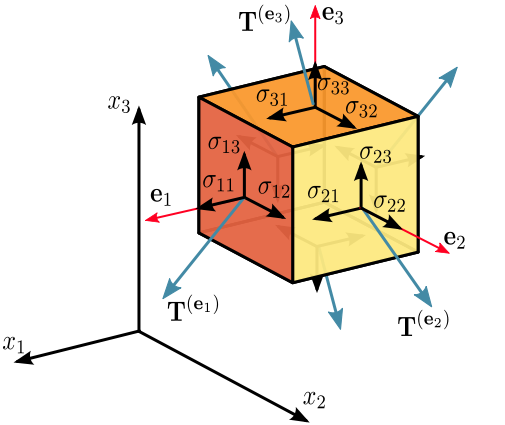
\includegraphics[width=0.6\textwidth]
    {img/stress_tensor.png}
  }
  \caption{Cauchy stress Tensor}
  \captionsetup{font={footnotesize,bf,it}}
  \caption*{src: \url{https://en.wikipedia.org/wiki/Cauchy_stress_tensor\#/media/File:Components_stress_tensor_cartesian.svg}}
  \label{cauchy}
\end{figure}

The Cauchy stress tensor, which is propably the classical example of a tensor, is depicted in Fig. \ref{cauchy} and consists of 3 stress vectors $\mathbf{T(e_i)}$, arranged in row-major order. It appears in similar form as viscous stress tensor in fluid mechanics:
\begin{align*}
\boldsymbol{\sigma}
 = \left[{\begin{matrix} \mathbf{T}^{(\mathbf{e}_1)} \\
\boldsymbol{T}^{(\mathbf{e}_2)} \\
\boldsymbol{T}^{(\mathbf{e}_3)} \\
\end{matrix}}\right] =
\left[{\begin{matrix}
\sigma _{xx} & \sigma _{xy} & \sigma _{xz} \\
\sigma _{yx} & \sigma _{yy} & \sigma _{yz} \\
\sigma _{zx} & \sigma _{zy} & \sigma _{zz} \\
\end{matrix}}\right]  = \left[{\begin{matrix}
\sigma _x & \tau _{xy} & \tau _{xz} \\
\tau _{yx} & \sigma _y & \tau _{yz} \\
\tau _{zx} & \tau _{zy} & \sigma _z \\
\end{matrix}}\right] =
\begin{bmatrix}
\sigma _{11} & \sigma _{12} & \sigma _{13} \\
\sigma _{21} & \sigma _{22} & \sigma _{23} \\
\sigma _{31} & \sigma _{32} & \sigma _{33} 
\end{bmatrix}.
\end{align*}
These 3 stress vectors represent the orientation and magnitude of total resulting stress at plane ${x,y,z}$ in plane normal directions ${x,y,z}$ ($3^2=9$ individual numbers). Thus, the stress tensor poses a full valid represenation of the stress distribution at any point in space. The stress tensor itself can be interpreted as a transformation, which maps an incoming normal direction vector $\mathbf{n}$ a resulting stress vector $\mathbf{T^{(n)}} = \mathbf{n}\cdot\boldsymbol{\sigma}$. The stresses in normal directions (diagonal elements) are directly related to the pressure, which is always isotropic and hence non-directionally dependent (kind of a Euclidean distance of the stress components). The tensor itself is a complicated representation and needs to be projected onto its principal axes to lower its dimensionality, as it is the case for principal component analysis. It is possible to find $2$ principal stress directions in $2D$ through PCA (see sect. \ref{sec:pca} below), for which there are no shear stresses existent in equilibrium. These form the principal directions of deformation at a certain location and are sufficient to describe the resulting transformation/deformation behaviour. The resulting system of principal directions and absolute stresses is often called an ``eigensystem'' or ``eigenframe''. So to say, an eigensystem, consistent of the principal directions/axes, spans a principal ellipsoid depicted in Fig. \ref{hat} in sect. \ref{sec:pca}. Another interpretation for the principal component ellipsoid is that it is the result of the tensor transformation applied to the unit circle. It is therefore somehow representing the distortion of an absolutely isotropic object (unit circle) by whatever the underlying affine tensor transformation effects (e.g. stretching, shearing, mirroring, scaling, rotating). Let us consider it as some lower dimensional, more intuitive representation of the tensor which we were left with in the first place. To put it all together, a tensor is a mathematical transformation which is encoded inside of an abstract $oD$ number array, which comes in need, whenever we have a whole distribution of directions manifesting itself inside of a tensor (matrix) transformation.

\section{Polar Coordinates}
\label{sec:polar}
\begin{figure}[!t]
  \centering
 {
    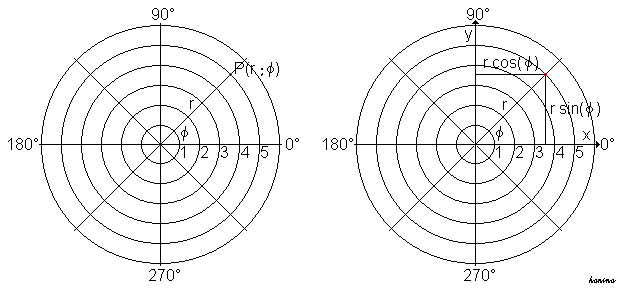
\includegraphics[width=0.8\textwidth]
    {img/polarkoordinaten.png}
  }
  \caption{polar space}
  \captionsetup{font={footnotesize,bf,it}}
   \caption*{src: \url{https://de.wikipedia.org/wiki/Datei:Ebene_polarkoordinaten.PNG}}
  \label{polar}
\end{figure}\vskip 3pt
Mathematically speaking, a polar space is a system, which maps each angle $\omega$ a magnitude $r(\omega)$ through a symbolic function. The conversion formula from polar (given a radius $r$ and angle $\omega$) to Cartesian coordinates is depicted in Fig. \ref{polar} and is given by:
\begin{align*}
	x &= r \cos \omega, \\
 	y &= r \sin \omega.
\end{align*}
Note, that we switched angle $\phi$ to $\omega$ for reasonable discrimination to the radiant intensity. The inverse direction (given coordinates $x,y$) is a bit more complicated:
\begin{align*}
	r &= \sqrt{x^2 + y^2} \\
\omega &= \operatorname{atan2}(y, x)
\end{align*}
The polar domain is a circular axis version of the domain $[0..2\pi]$, with negative magnitudes in $r$ shifted by 180 degrees (point reflected) as this is the formal behaviour defined and required by the conversion formulas.

\section{Principal Component Analysis}
\label{sec:pca}
Note, that we denote a matrix with a second order tensor interchangeably for the sake of simplicity in the following. Also keep in mind, that we interpret a matrix or tensor as affine transformation. For any state of stress in equilibrium it is possible to find $n$ (dimensionality) independent orthogonal directions with no shear stresses existent. Along these directions the principal stresses, which are normal (tensile/compressive) stresses, are exerted. The anisotropy can be represented by, e.g., ellipsoid glyphs.

\begin{figure}[!t]
\hskip 22pt
  \begin{minipage}[!t]{0.4\textwidth}
    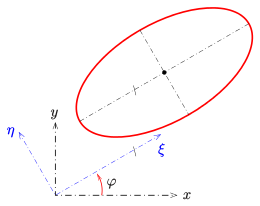
\includegraphics[width=\textwidth]{img/HAT.png}
   \caption{2D principal component ellipsoid\/ glyph (eigenframe)}
   \label{hat}
   \captionsetup{font={footnotesize,bf,it}}
   \caption*{src: \url{https://de.wikipedia.org/wiki/Datei:HAT-ellipse0.svg}}
  \end{minipage} \hskip 40pt
  %\raggedright
  \begin{minipage}[!t]{0.4\textwidth}
    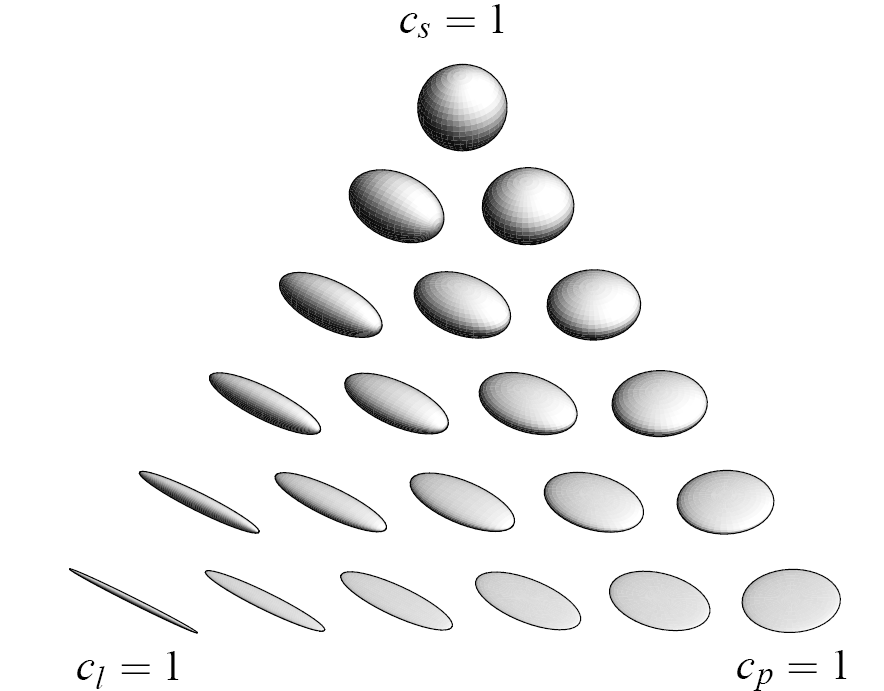
\includegraphics[width=\textwidth]{img/glyphs.png}
    \caption{3D ellipsoid glyphs w. anisotropy coefficient (l:linear, p:planar, s:spherical)}
    \label{3Dglyphs}
    \captionsetup{font={footnotesize,bf,it}}
   \caption*{src: \url{https://slideplayer.com/slide/5291764/}}
  \end{minipage}
\end{figure}

Principal Component Analysis is an algorithm, which is able to capture the principal components (directions) in stochastic data. But it works similarly on transformations to capture the principal directions from transformations like rotation and scaling. Now, principal component analysis can be done by eigenvalue or singular vector decomposition, whereas the former yields complex eigenvalues for asymmetric matrices. For (skew-) symmetric (normal) matrices, they are connected through the following relation: $s_i = \sqrt{|\lambda_i|}$ (cf. \cite{kieburg}). Note, that the eigenvectors match the singular vectors only for symmetric matrices, which does not mean that they do not form the half-axes of the principal component ellipsoid in other cases (cf. \cite{moler}). Mathematically speaking, a decomposition is somehow decomposing a transformation (which follows certain transformation rules) into parts of subsequent transformations consistent of rotation and scaling (classically: $\mathbf{A} = \mathbf{R}\mathbf{S}\mathbf{R}^*$). We choose to use singular value decomposition ($\mathbf{A} = \mathbf{U} \mathbf{\Sigma} \mathbf{V}^*$) to be able to set up real eigenvalues for any kind of matrix (singular values are always real and positive). Also, the singular vectors of the $\mathbf{U}$-matrix represent the half-axes of the principal ellipsoid (eigenframe) shown in Fig. \ref{HAT} for any kind of transformation matrix. The singular value decomposition is defined as follows:
\begin{align*}
	\mathbf{A} = \mathbf{U} \boldsymbol{\Sigma} \mathbf{V}
\end{align*}
where
\begin{itemize}
	\item $\mathbf{U}$ is an $m × m$ unitary matrix
	\item $\boldsymbol{\Sigma}$ is a diagonal matrix {$m × n$} with positive real numbers on the diagonal
	\item $\mathbf{V}$ is an {$n × n$} unitary matrix, $\mathbf{V}^*$ is its conjugate transpose
\end{itemize}
 
In addition, we also calculate the eigenvalues to exploit the sign of the real part of the eigenvalues (\cite{mroz}) ordered decreasingly by absolute value (corresponding to singular value order). The sign corresponds to tensile ($+$) and compressive ($-$) stress, which would allow us to visualize deformation glyphs with arrows pointing inwards for compressive and outwards for tensile stresses. We do this decomposition analysis once for each matrix and then store the precomputed results in a grid. The principal ellipsoid is also used as a transmission profile for the propagation scheme in symbolic form in a subequent step, which makes it a basic and central concept within the scope of this work. Within this work, we will use the singular vectors yielded from singular value decomposition to avoid complex values yielded from eigenvalue decomposition. This will allow us to set up glyphs representing the major/minor axis of the underlying transformation for every kind of (asymmetric/symmetric) tensor. We will then use global-illumination techniques on top to generate a light transport flow map, which permits us somehow to forward the intensities which are given as predefined initialization values in form of symbolic functions defined by the user. This kind of light transport propagation scheme will also allow us to compute an FTLE-like field on the tensor fields.

\section{Finite-Time Lyapunov Exponent}
\label{sec:ftle}
The Finite-Time Lyapunov Exponent is a measure, developed to analyze time-dependent dynamical systems for their separation abilities concerning massless tracer particles. We imagine a flow field, i.e., a vector field which in turn represents the effective amount or concentration shifted into a particular direction at each point in space. It could induced by e.g. concentration or height gradients. This flow field is considered a time-dependent dynamical system, since it usually holds a time-component $t$ and thus maps each initial position an aged (altered) position: $\mathbf{\upvarphi}(\mathbf{x}) : \mathbf{x}(t_0) \longmapsto \mathbf{x}(t_0+T)$. We can now imagine placing two close by particles in distance $\delta$ into a flow field and run a time dependent simulation. Remark that this corresponds to the Lagrangian view in vector fields, which travels with the particles (instead of taking the position of a resting observer - Eulerian view):

\begin{figure}[!t]
  \centering
 {
    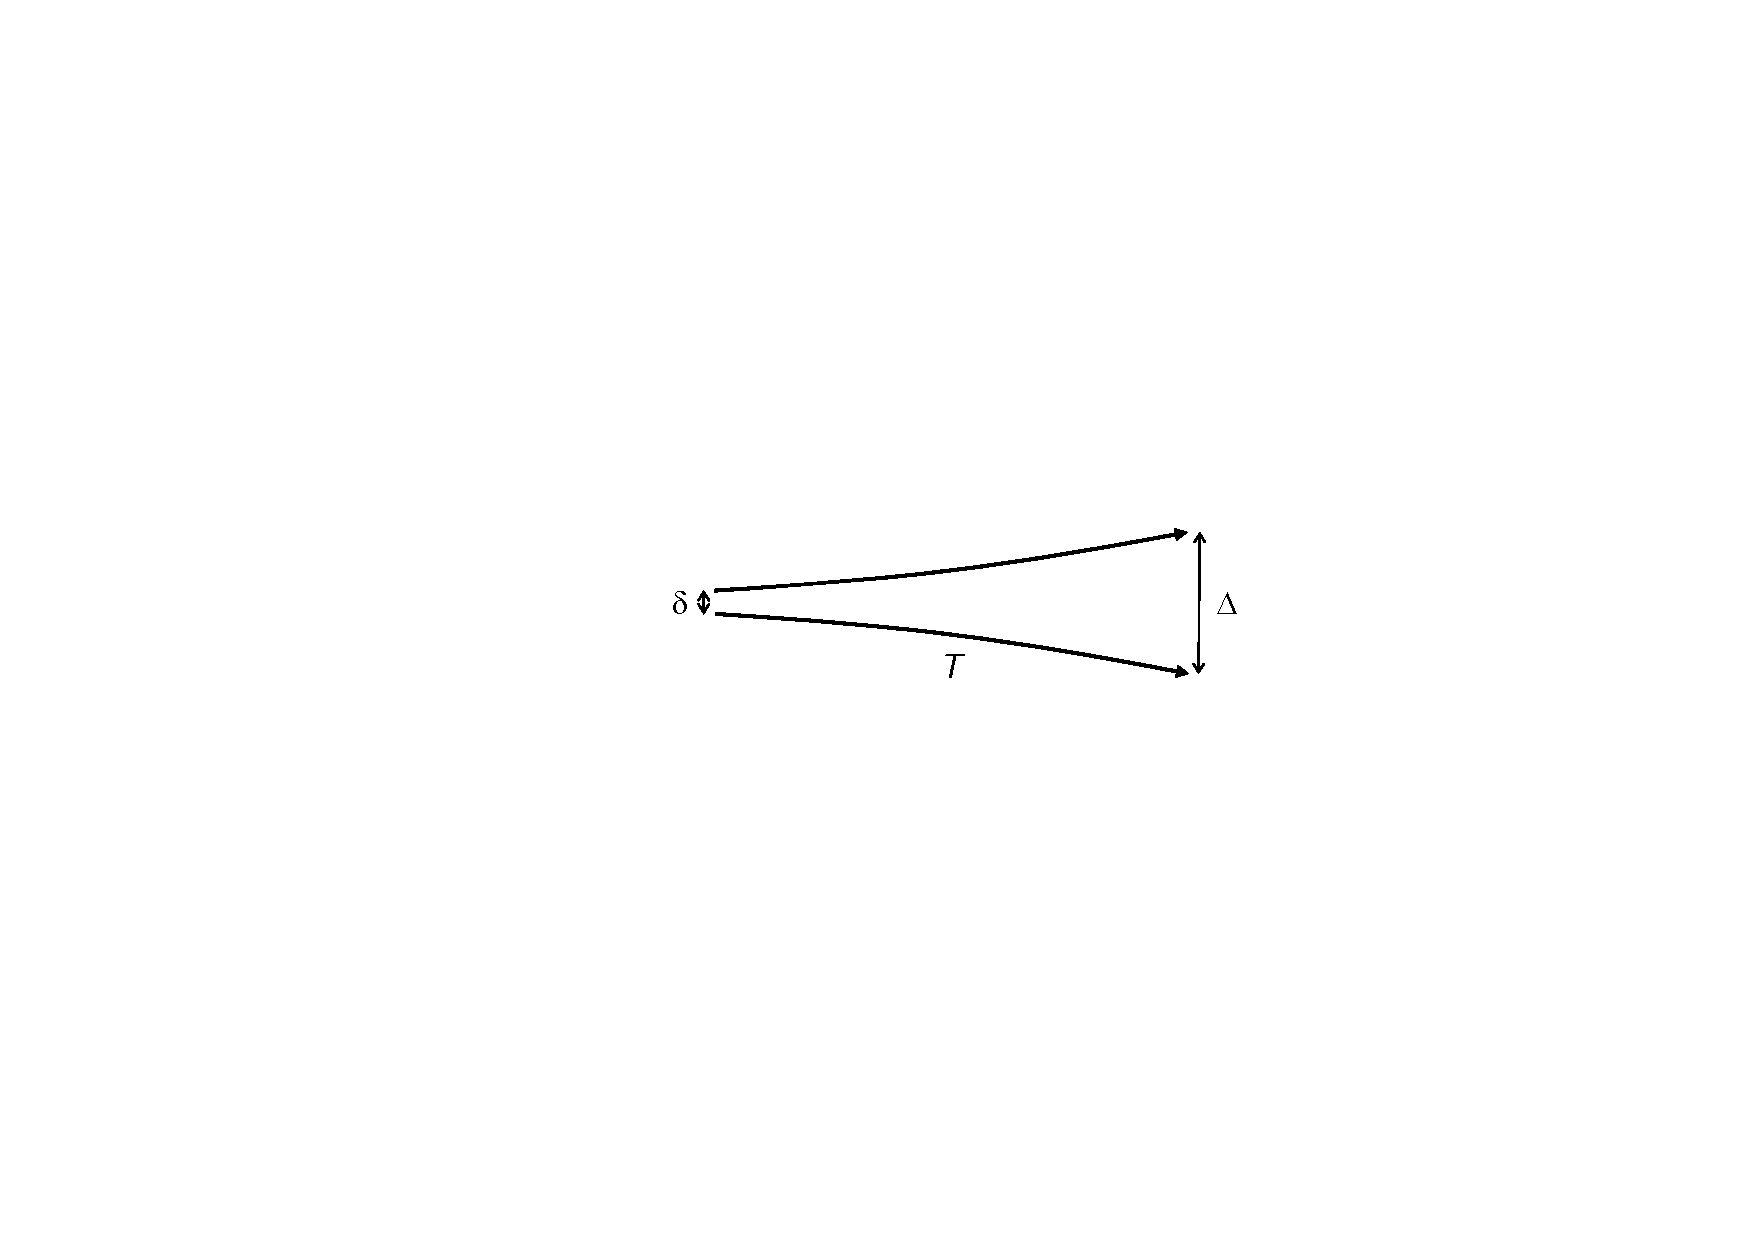
\includegraphics[width=0.6\textwidth]
    {img/ftle_sep.pdf}
  }
  \caption{FTLE: separation of massless tracer particles}
  \captionsetup{font={footnotesize,bf,it}}
  \caption*{src: Skript Prof. Sadlo, Scientific Visualization SS2017, Heidelberg University}
  \label{ftle_sep}
\end{figure}

We observe particle trajectories diverging w.r.t. the central axis ending up in distance $\Delta$. The FTLE measure for this single example (point in space) is then defined as:

\begin{align*}
	\sigma = \frac{1}{\lvert T\rvert}\ln \frac{\Delta}{\delta}
\end{align*}

Alternatively, an FTLE can also be computed from a flow map's gradient, which is more convenient to compute in general:
\begin{align*}
	\sigma(\mathbf{x})=\frac{1}{\lvert T\rvert}\ln \lvert\lvert\nabla\mathbf{\upvarphi(x)}\rvert\rvert _2,
\end{align*}
whereas $\lvert\lvert A\rvert\rvert _2 = \sqrt{\lambda_{max}(A^TA)}$ is the spectral norm of matrix $A$. This will yield a map, which responds most where path lines diverge w.r.t. to a central axis. We consider an example which detects FTLE ridges inside of the cross-section of a double gyre. Note, that this example considers single trajectories diverging implicitly:
\begin{figure}[!t]
\hskip 22pt
  \begin{minipage}[!t]{0.4\textwidth}
    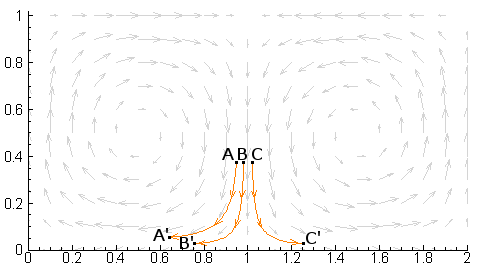
\includegraphics[width=\textwidth]{img/diverge.png}
   \caption{diverging streamlines for double gyre}
   \label{diverge}
   \captionsetup{font={footnotesize,bf,it}}
   \caption*{src: \url{https://shaddenlab.berkeley.edu/uploads/LCS-tutorial/dg_3traj.png}}
  \end{minipage} \hskip 40pt
  %\raggedright
  \begin{minipage}[!t]{0.4\textwidth}
    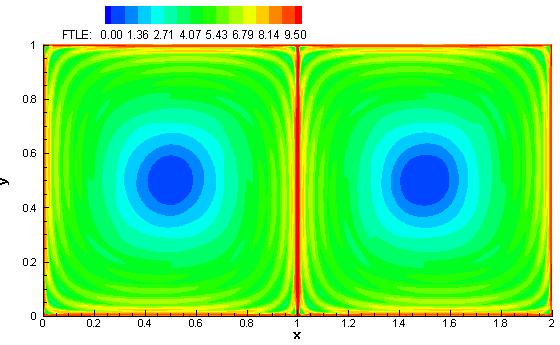
\includegraphics[width=\textwidth]{img/ftle_gyre.png}
    \caption{FTLE field for double gyre}
    \label{ftle_gyre}
    \captionsetup{font={footnotesize,bf,it}}
   \caption*{src: \url{https://shaddenlab.berkeley.edu/uploads/LCS-tutorial/dle_incT.png}}
  \end{minipage}
\end{figure}
Fig \ref{diverge} and \ref{ftle_gyre} depict a scenario of diverging streamlines for a double gyre snapshot in time (yielding a time-independent dynamical system). Fig. \ref{ftle_gyre} features a high ridge on the margins (borders) and in particular at the center of the domain. This region of interest (ROI) is considered to indicate the maximum relative local divergence of tensor field lines, by the approach. Ridges also represent Lagrangian Coherent Structures, which are found in nature in vortices of correlating flow behavior.  We could imagine to introduce this process for a whole distribution of trajectories, which would implement an FTLE for uncertain vector fields in a sense, that whole propability distributions of trajectories could be heeded. An overview about existing visualization techniques for uncertain data is given by Griete \& Schuhmann \cite{griete}. We require that the trajectories can cross each other unaffectedly, i.e., the superposition principle is supposed to be respected for the magnitudes. But behold, is this behavior not somehow familiar? If we elaborately think this through, we can come up with the idea that this is the behavior of light propagation in vacuum. Light paths are physically allowed to cross each other with no influence exerted on each other at all. Consequently, we choose to model the distributions of trajectories as light intensity profiles. That is, we interpret the polar profiles as a propability density function (PDF) for particle trajectories heading into this direction. To put it into context, our main contribution method LTG uses the FTLE as an inspiration or template to design a similar approach for tensor field visualization. The main difference to the template FTLE is that we follow eigenvectors instead of flow vectors and that we use whole distributions of trajectories, as a tensor field suggests whole distributions of directions, accordingly.

\section{GT Datasets / Methods}
\label{sec:gt}
\paragraph{Glyphs and Tensor Field Lines}
\begin{figure}[!t]
  \centering
 {
    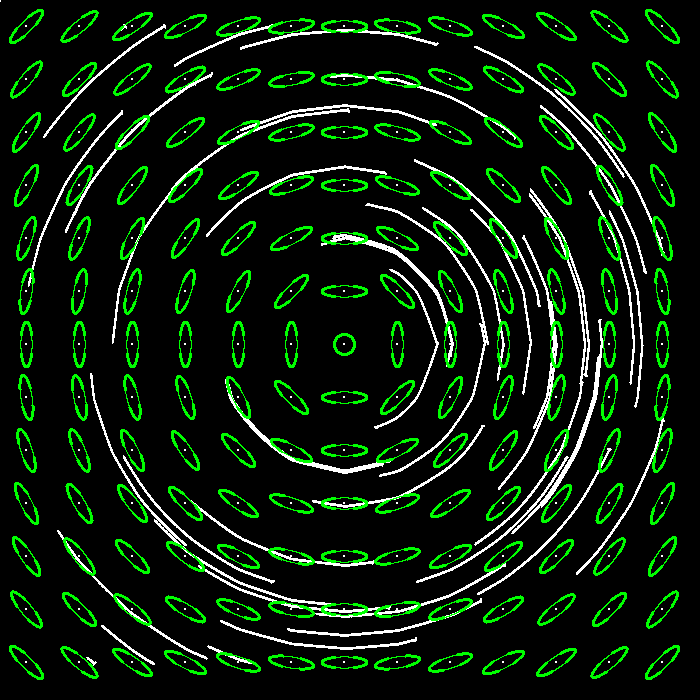
\includegraphics[width=0.4\textwidth]
    {img/tensorfieldlines.png}
  }
  \caption{tensor field lines: bold lines; ellipsoids: ellipsoid glyphs}
  \label{scheme}
\end{figure}\vskip 3pt
Glyphs are derived as a basis for the weighting profiles of the tensors in the following propagation scheme. They were chosen because it is an easy-to-use (understand) concept, which can also be interpreted nicely. In fact, these representations are used for the principal component analysis of direction vectors for the tensor field line extrapolation (integration) and also as transmission profiles for the light propagation scheme in a subsequent step. We can again emphasize glyphs as a crucial, central concept within this work. Tensor field lines (the type of tensor streamline analog that does not introduce artificial intertia) were implemented for ground truth (GT) data generation purposes. For example, when designing a FTLE-like field computation technique, we will need to know when tensor field lines diverge/converge.

\paragraph{Test Data (Generation)}
We used python's numpy library to generate predefined, synthetic test cases and caught two real data example from \url{TensorVis.org} and \url{https://www.cs.purdue.edu/homes/cs530/projects/project5.html}, which needed to be pre-processed through slicing and subsequent cropping to obtain $2D$ samples ($2\times2$) matrices). These test fields can be grouped into symmetric and asymmetric ones:\\

\begin{figure}[!t]
\centering
  \begin{minipage}{0.3\textwidth}
    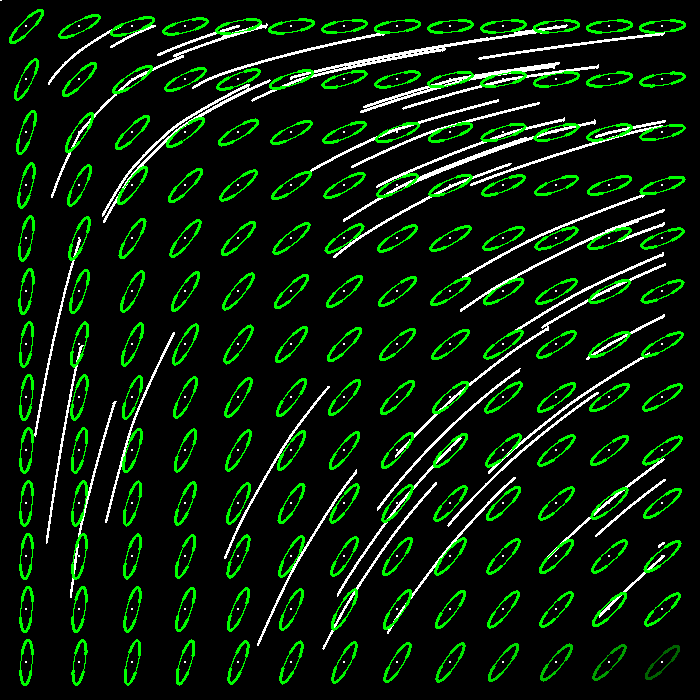
\includegraphics[height=\textwidth]{img/corner-TFL.png}
    \caption{``corner'' test field}
    \label{a)}
  \end{minipage}
  \begin{minipage}{0.3\textwidth}
    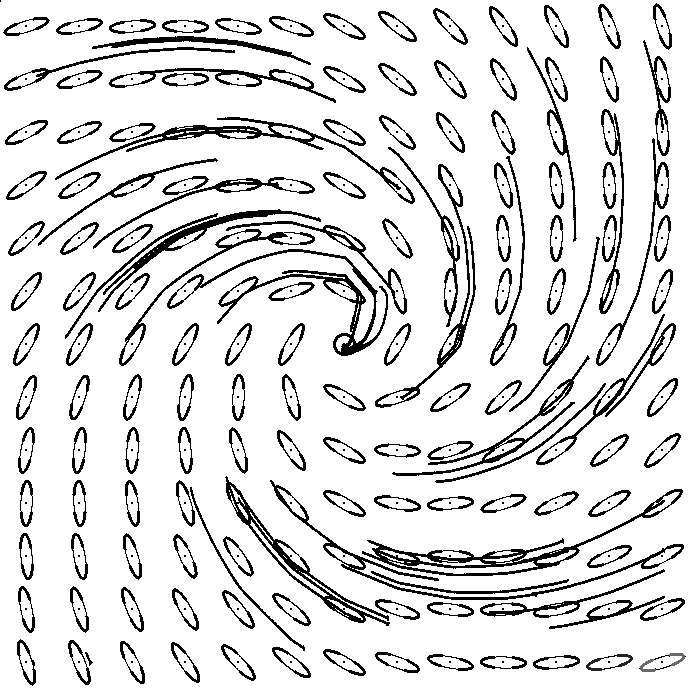
\includegraphics[height=\textwidth]{img/spiral-TFL.png}
    \caption{``spiral'' test field}
    \label{b)}
  \end{minipage}
  \begin{minipage}{0.3\textwidth}
    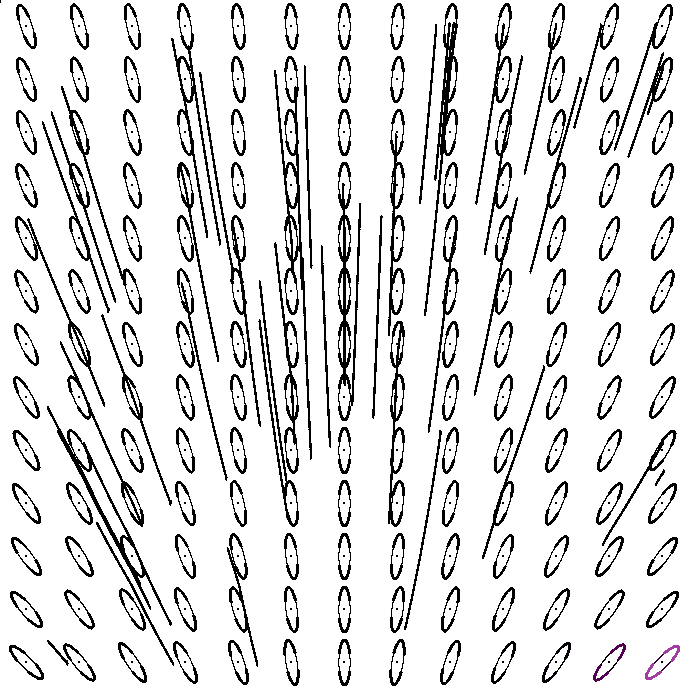
\includegraphics[height=\textwidth]{img/drain_old.png}
    \caption{``V'' test field    }
    \label{b)}
  \end{minipage}
%\caption{a) , b) , c) }
\label{test-fields}
\end{figure}

\textbf{Symmteric Tensor Fields}
We also aim to use a real data example of the $3D$ DTI-MRI diffusion tensor of the brain for a male subject at the age of 27 and another one featuring a human heart. As we visualize 2D symmetric second order tensor fields, we need to slice the dataset and crop the $2{\times}2$ matrices omitting the $z$-component of the original $3{\times}3$ matrices. Fig. \ref{brainglyphs} depicts the glyph representation of the test dataset for slice index $8$:
\begin{figure}[!t]
\centering
  \begin{minipage}{0.4\textwidth}
    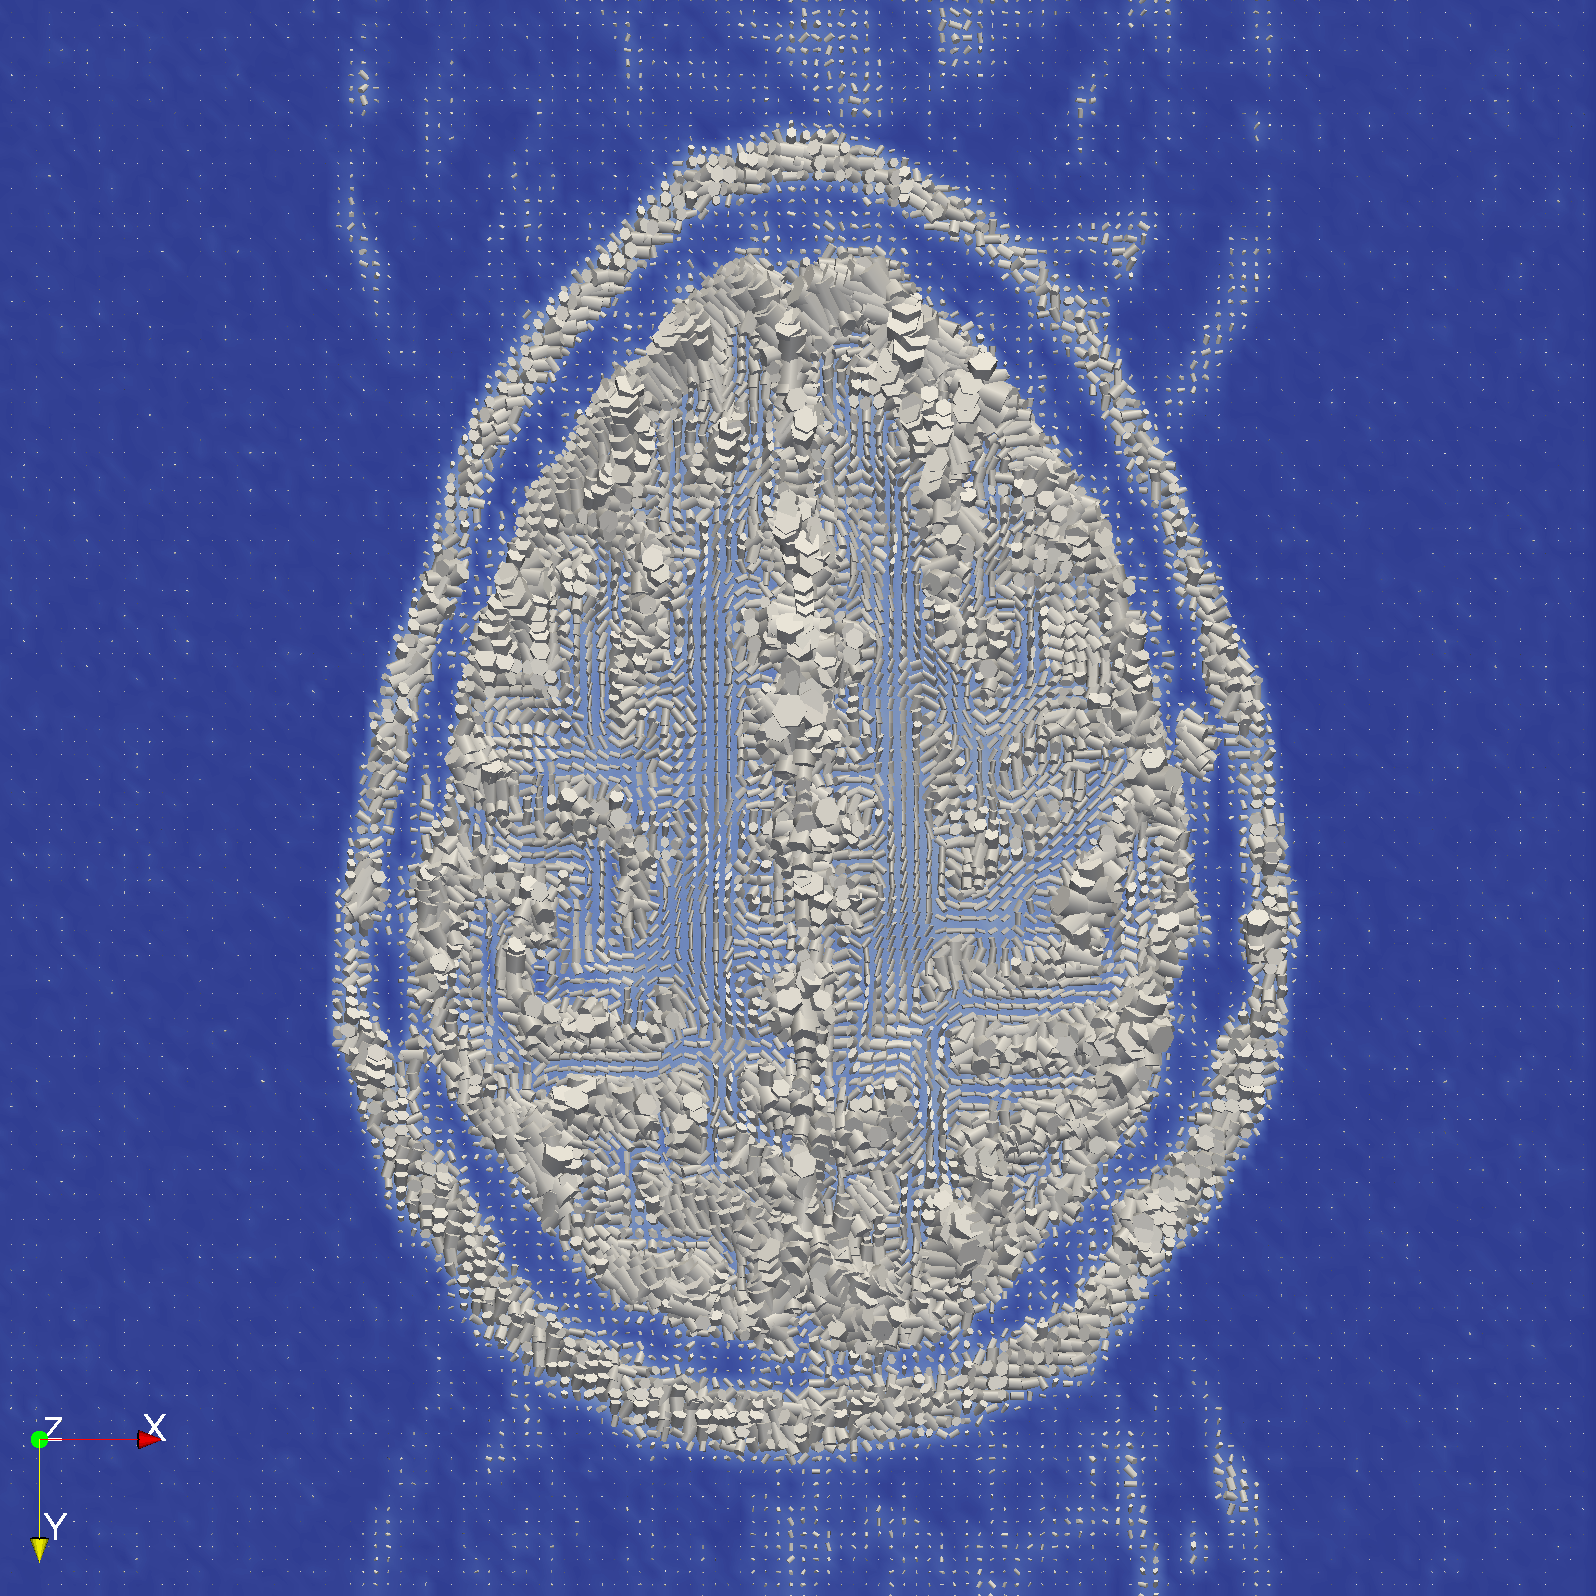
\includegraphics[width=\textwidth]{img/brain_cyl_glyphs.png}
    \label{a)}
    \caption*{cylinder glyphs}
  \end{minipage}
  \begin{minipage}{0.4\textwidth}
    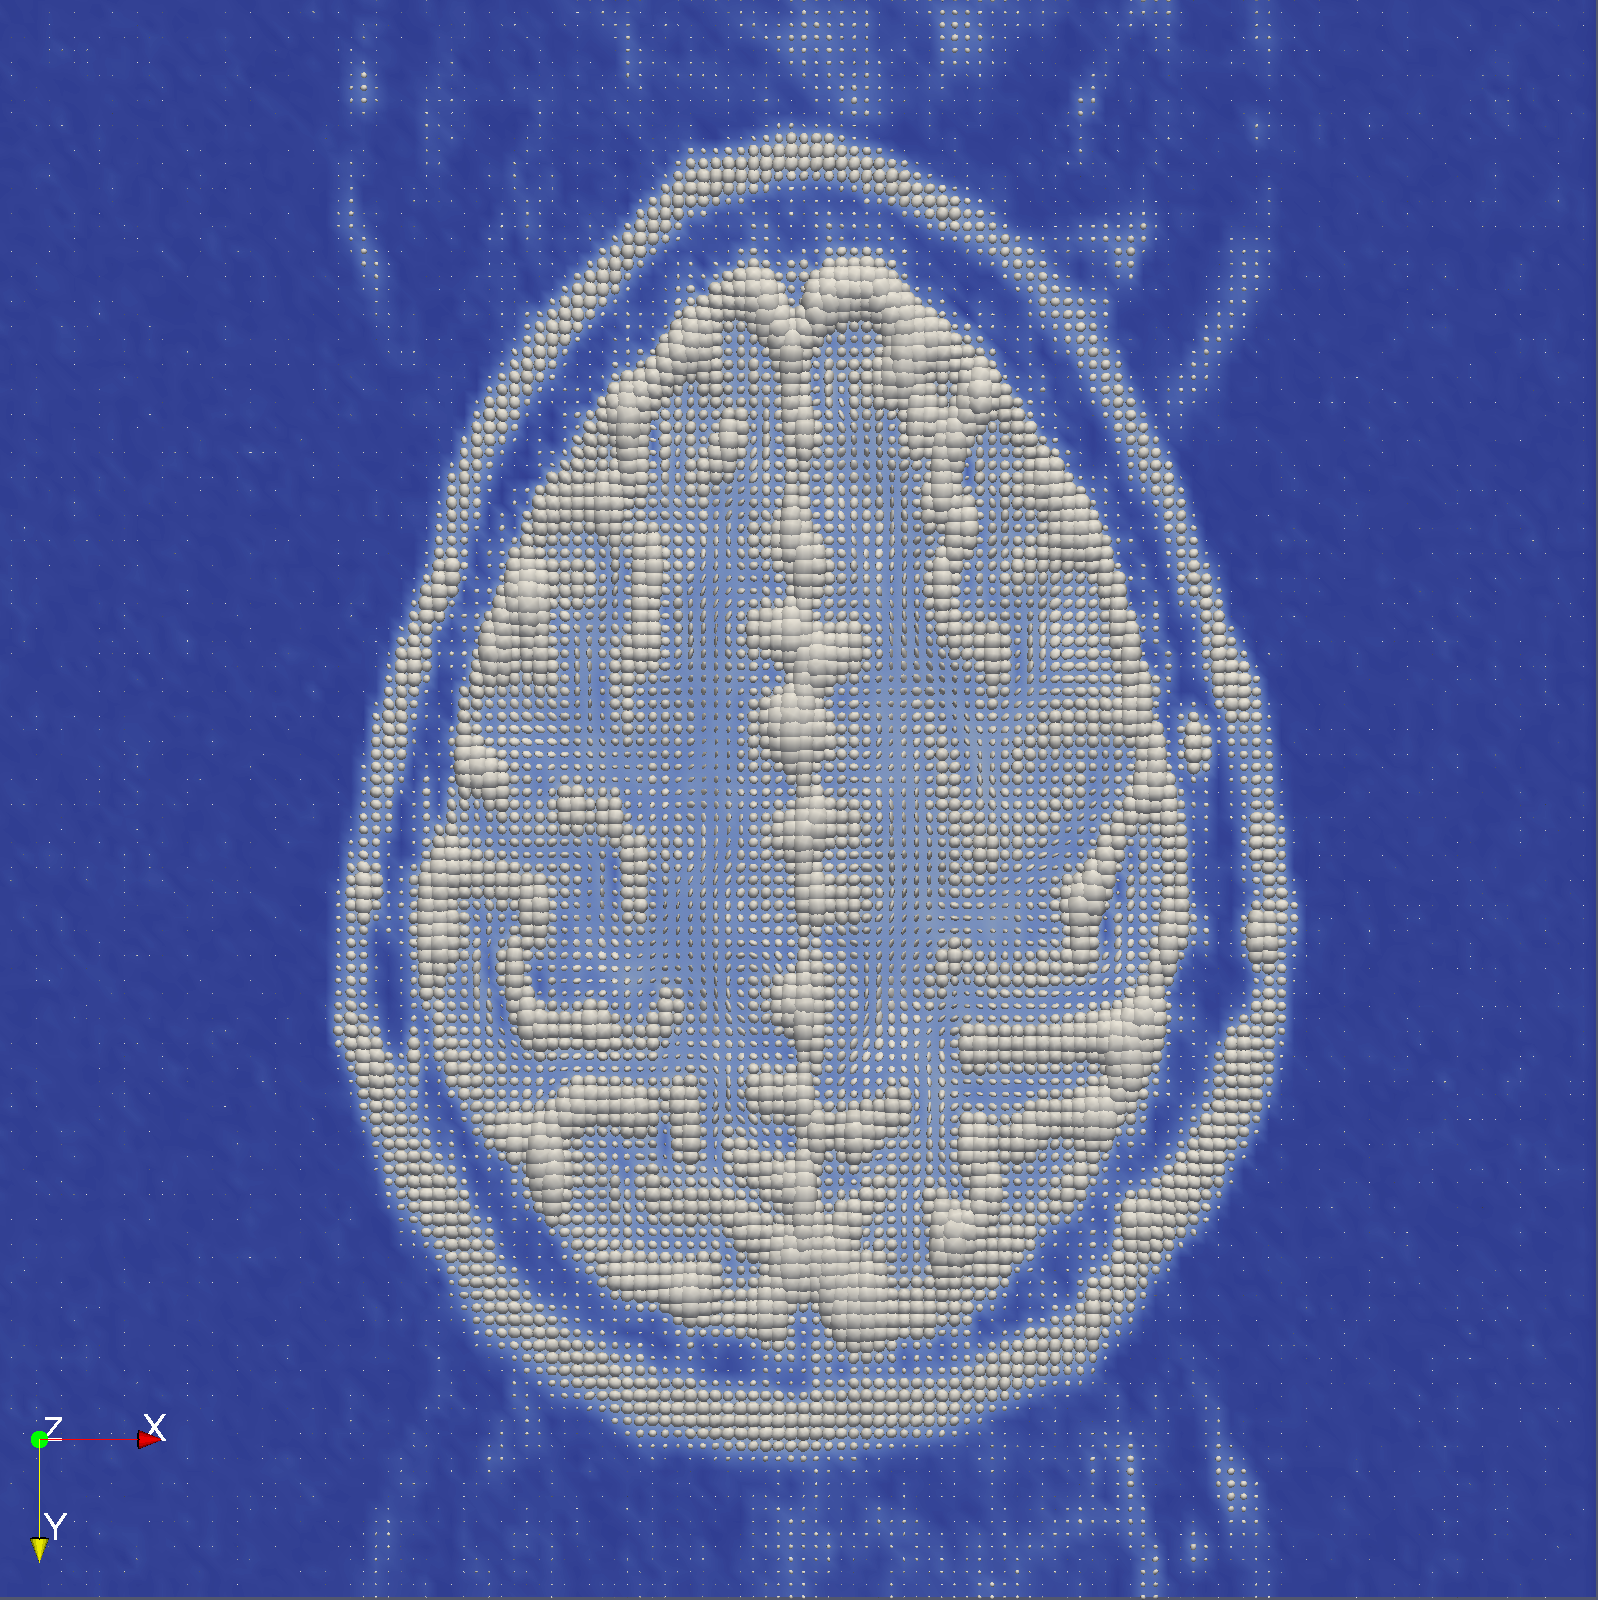
\includegraphics[width=\textwidth]{img/brain_ellipsoid_glyphs.png}
    \label{b)}
    \caption*{ellipsoid glyphs}
  \end{minipage}
\caption{``brain''-test field}
\label{brainglyphs}
\end{figure}


\textbf{Asymmetric Tensor Fields}

\begin{figure}[!t]
\centering
  \begin{minipage}{0.4\textwidth}
    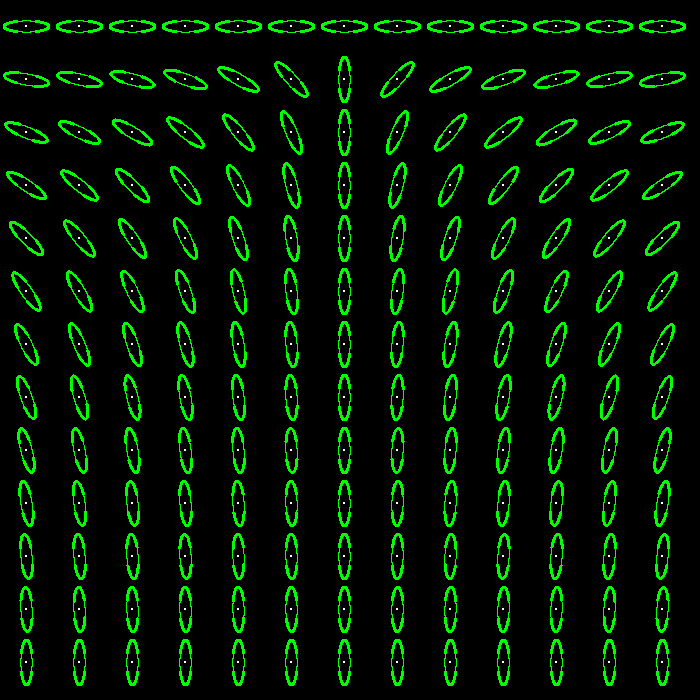
\includegraphics[width=\textwidth]{img/drain(alt).png}
    \label{a)}
  \end{minipage}
  \begin{minipage}{0.4\textwidth}
    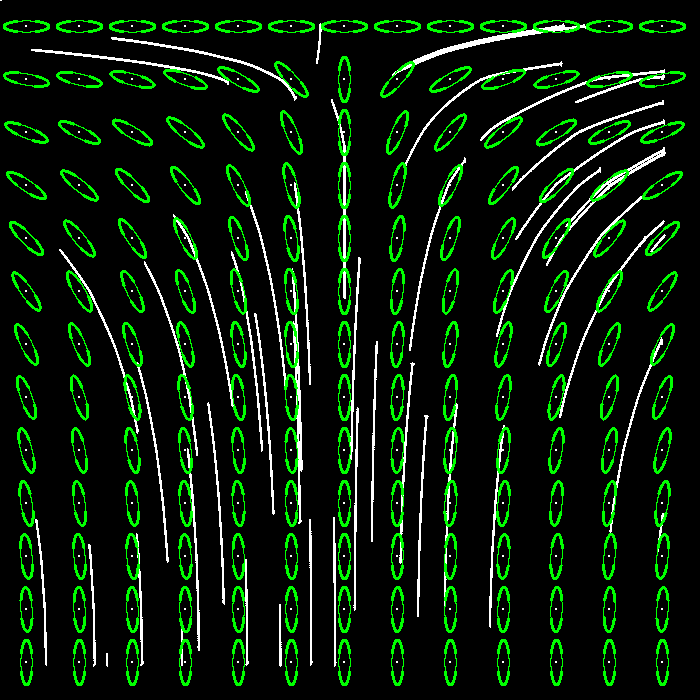
\includegraphics[width=\textwidth]{img/drain(alt)-TFL.png}
    \label{b)}
  \end{minipage}
\caption{a) ``drain''-testfield, b) tensor field lines for a)}
\label{drain}
\end{figure}

The ``drain''-Testfield, depicted in Fig. \ref{drain} is generated to have a kind of proof-of-concept (POC) for the FTLE-related approach. It poses raw, bare diverging tensor field lines without any other feature modulated on top. Thus, it can be expected to induce a high FTLE response, since it is an interpretable ground truth test and is considered to be a basic trigger/stimulus for the approach with no side effects introduced.

\begin{figure}[!t]
\centering
  \begin{minipage}{0.4\textwidth}
    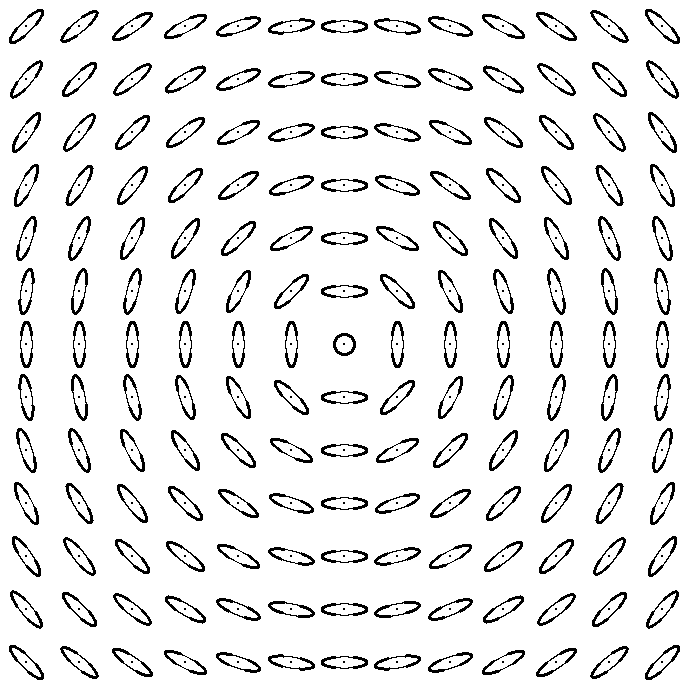
\includegraphics[width=0.8\textwidth]{img/rings.png}
    \label{a)}
  \end{minipage}
  \begin{minipage}{0.4\textwidth}
    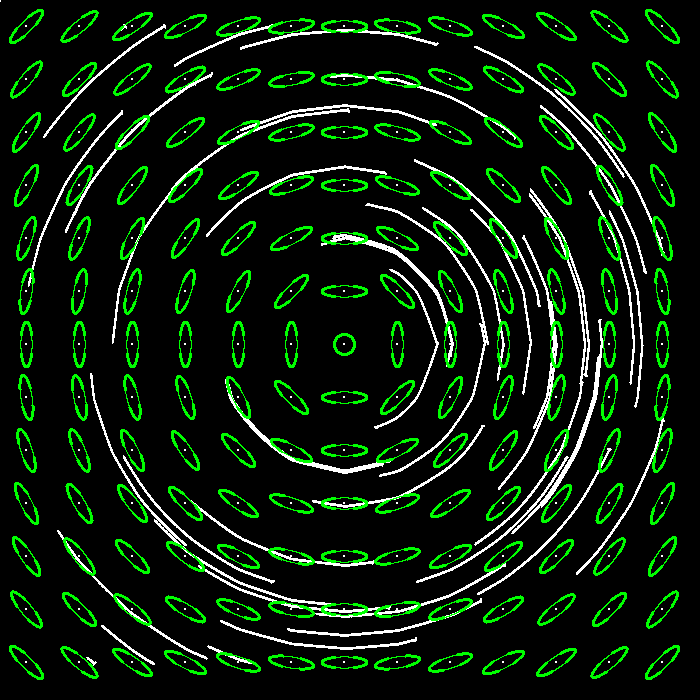
\includegraphics[width=0.8\textwidth]{img/tensorfieldlines.png}
    \label{b)}
  \end{minipage}
\caption{a) ``rings'' test field, b) tensor field lines for a)}
\label{rings}
\end{figure}
The ``rings'' test field, depicted in Fig. \ref{rings} should be used to demonstrate the directive ability of the approach transmitting energy in circular orbits.
\begin{figure}[!t]
\centering
  \begin{minipage}{0.4\textwidth}
    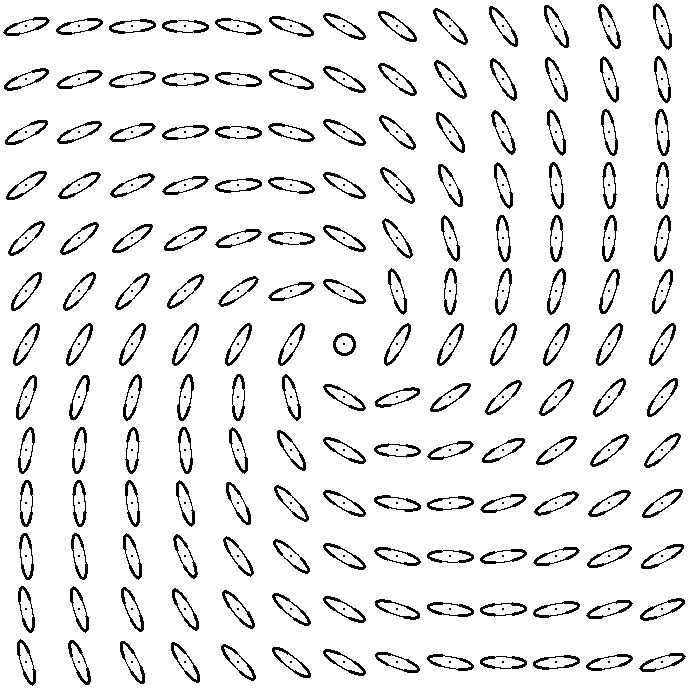
\includegraphics[width=0.8\textwidth]{img/spiral.png}
    \label{a)}
  \end{minipage}
  \begin{minipage}{0.4\textwidth}
    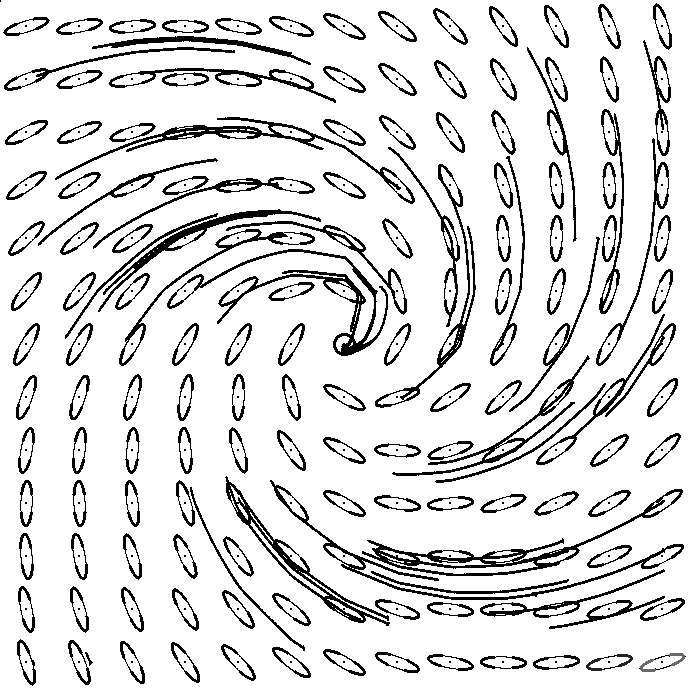
\includegraphics[width=0.8\textwidth]{img/spiral-TFL.png}
    \label{b)}
  \end{minipage}
\caption{a) ``spiral''-test field, b) tensor field lines for a)}
\label{spiral}
\end{figure}
The ``spiral'' test field, depicted in Fig. \ref{spiral} should be used to demonstrate the directive ability of the approach transmitting energy in archimedian spiral orbits.
\begin{figure}[!t]
\centering
  \begin{minipage}{0.4\textwidth}
    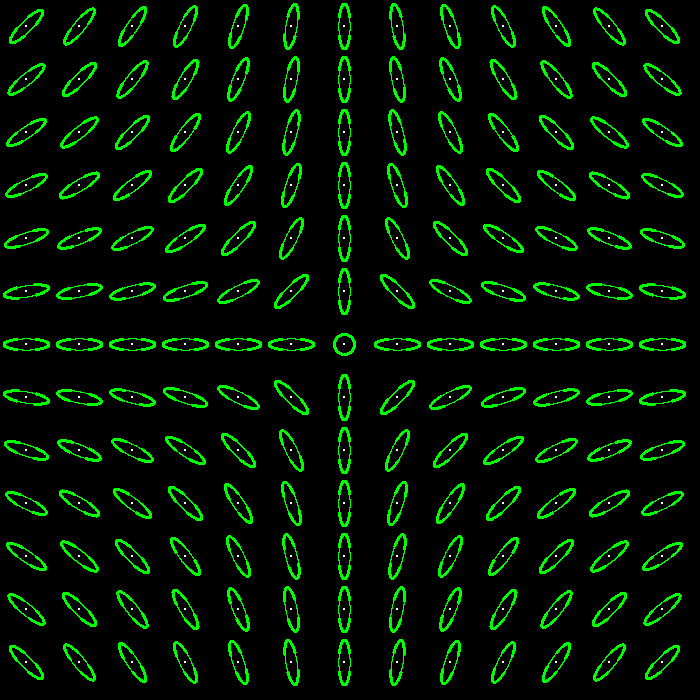
\includegraphics[width=0.8\textwidth]{img/inverse.png}
    \label{a)}
  \end{minipage}
  \begin{minipage}{0.4\textwidth}
    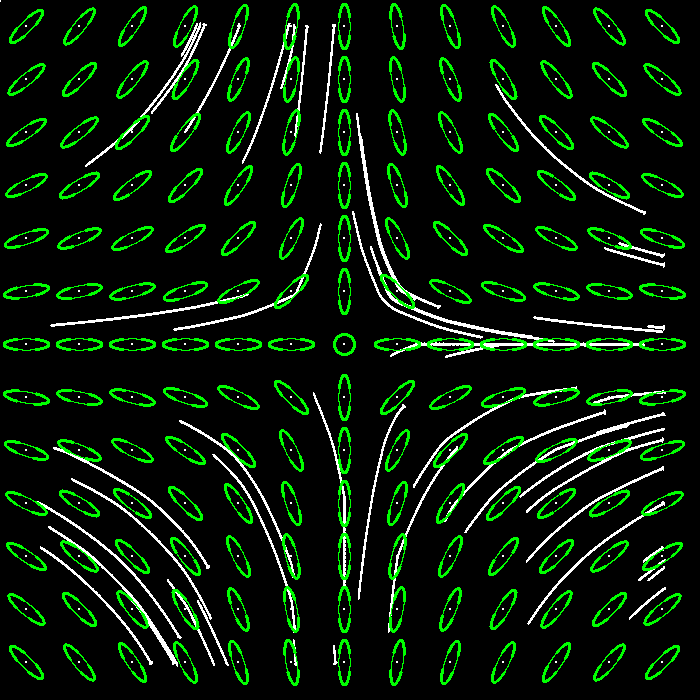
\includegraphics[width=0.8\textwidth]{img/inverse-TFL.png}
    \label{b)}
  \end{minipage}
\caption{a) ``inverse''-test field, b) tensor field lines for a)}
\label{inverse}
\end{figure}
With the \enquote{inverse} test field we want to demonstrate the directive separation of intensities into four quadrants.


\begin{figure}[!t]
\centering
  \begin{minipage}{0.4\textwidth}
    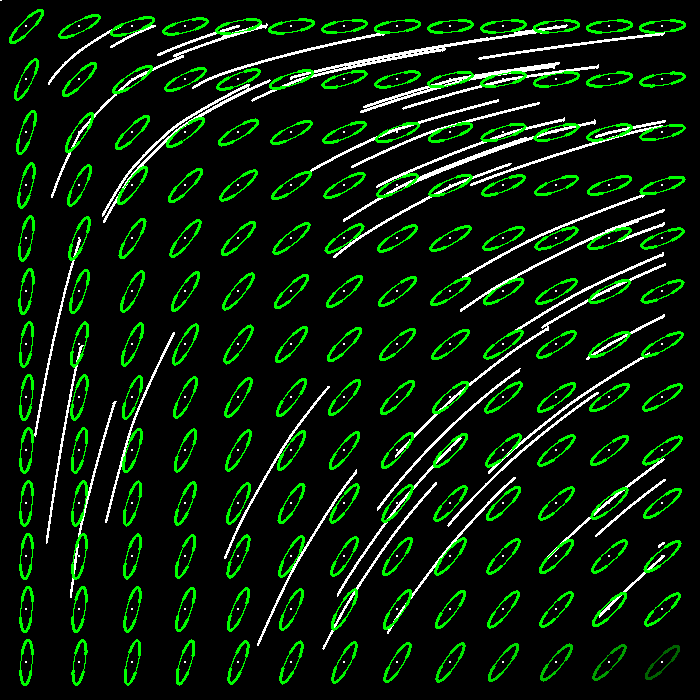
\includegraphics[width=0.8\textwidth]{img/corner.png}
    \label{a)}
  \end{minipage}
  \begin{minipage}{0.4\textwidth}
    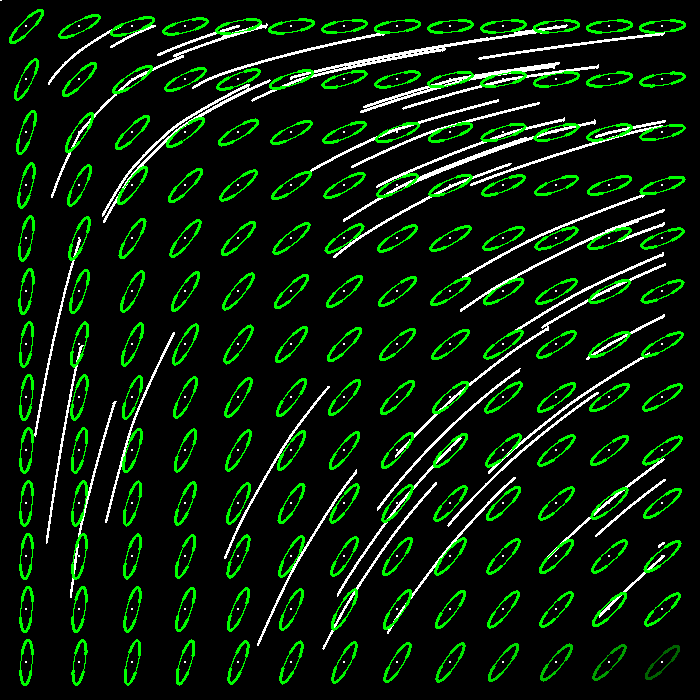
\includegraphics[width=0.8\textwidth]{img/corner-TFL.png}
    \label{b)}
  \end{minipage}
\caption{a) ``corner''-test field, b) tensor field lines for a)}
\label{corner}
\end{figure}
The test field ``corner'', depicted in Fig \ref{corner}, constitutes a sustained turn over the grid representing the redirection or forwarding along domain corners. To have some real examples involved, we apply the invented technique to both DTI-MRI \enquote{brain} and \enquote{heart} scans, which can be observed in Fig. \ref{real1}.
\begin{figure}[!t]
\centering
  \begin{minipage}{0.4\textwidth}
    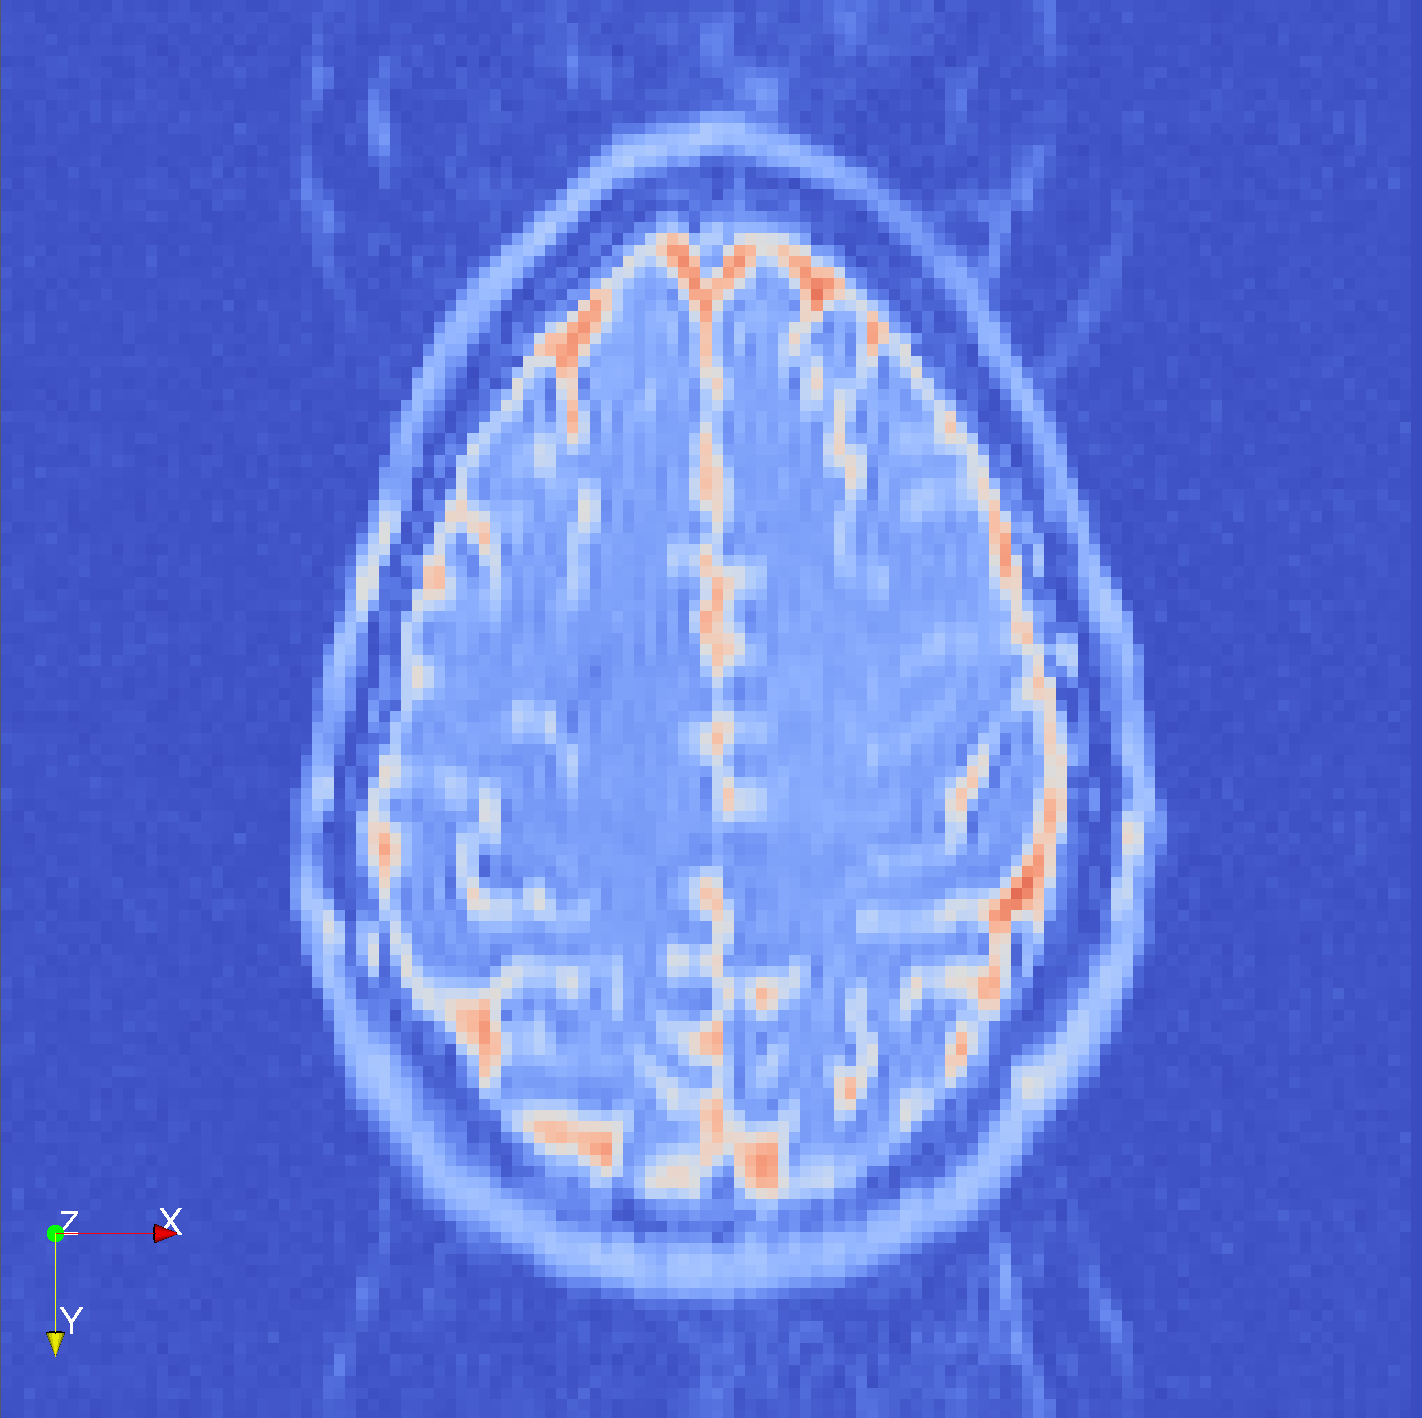
\includegraphics[width=0.8\textwidth]{img/brain_org.png}
    \label{a)}
    \caption*{tensor magnitude}
  \end{minipage}
  \begin{minipage}{0.4\textwidth}
    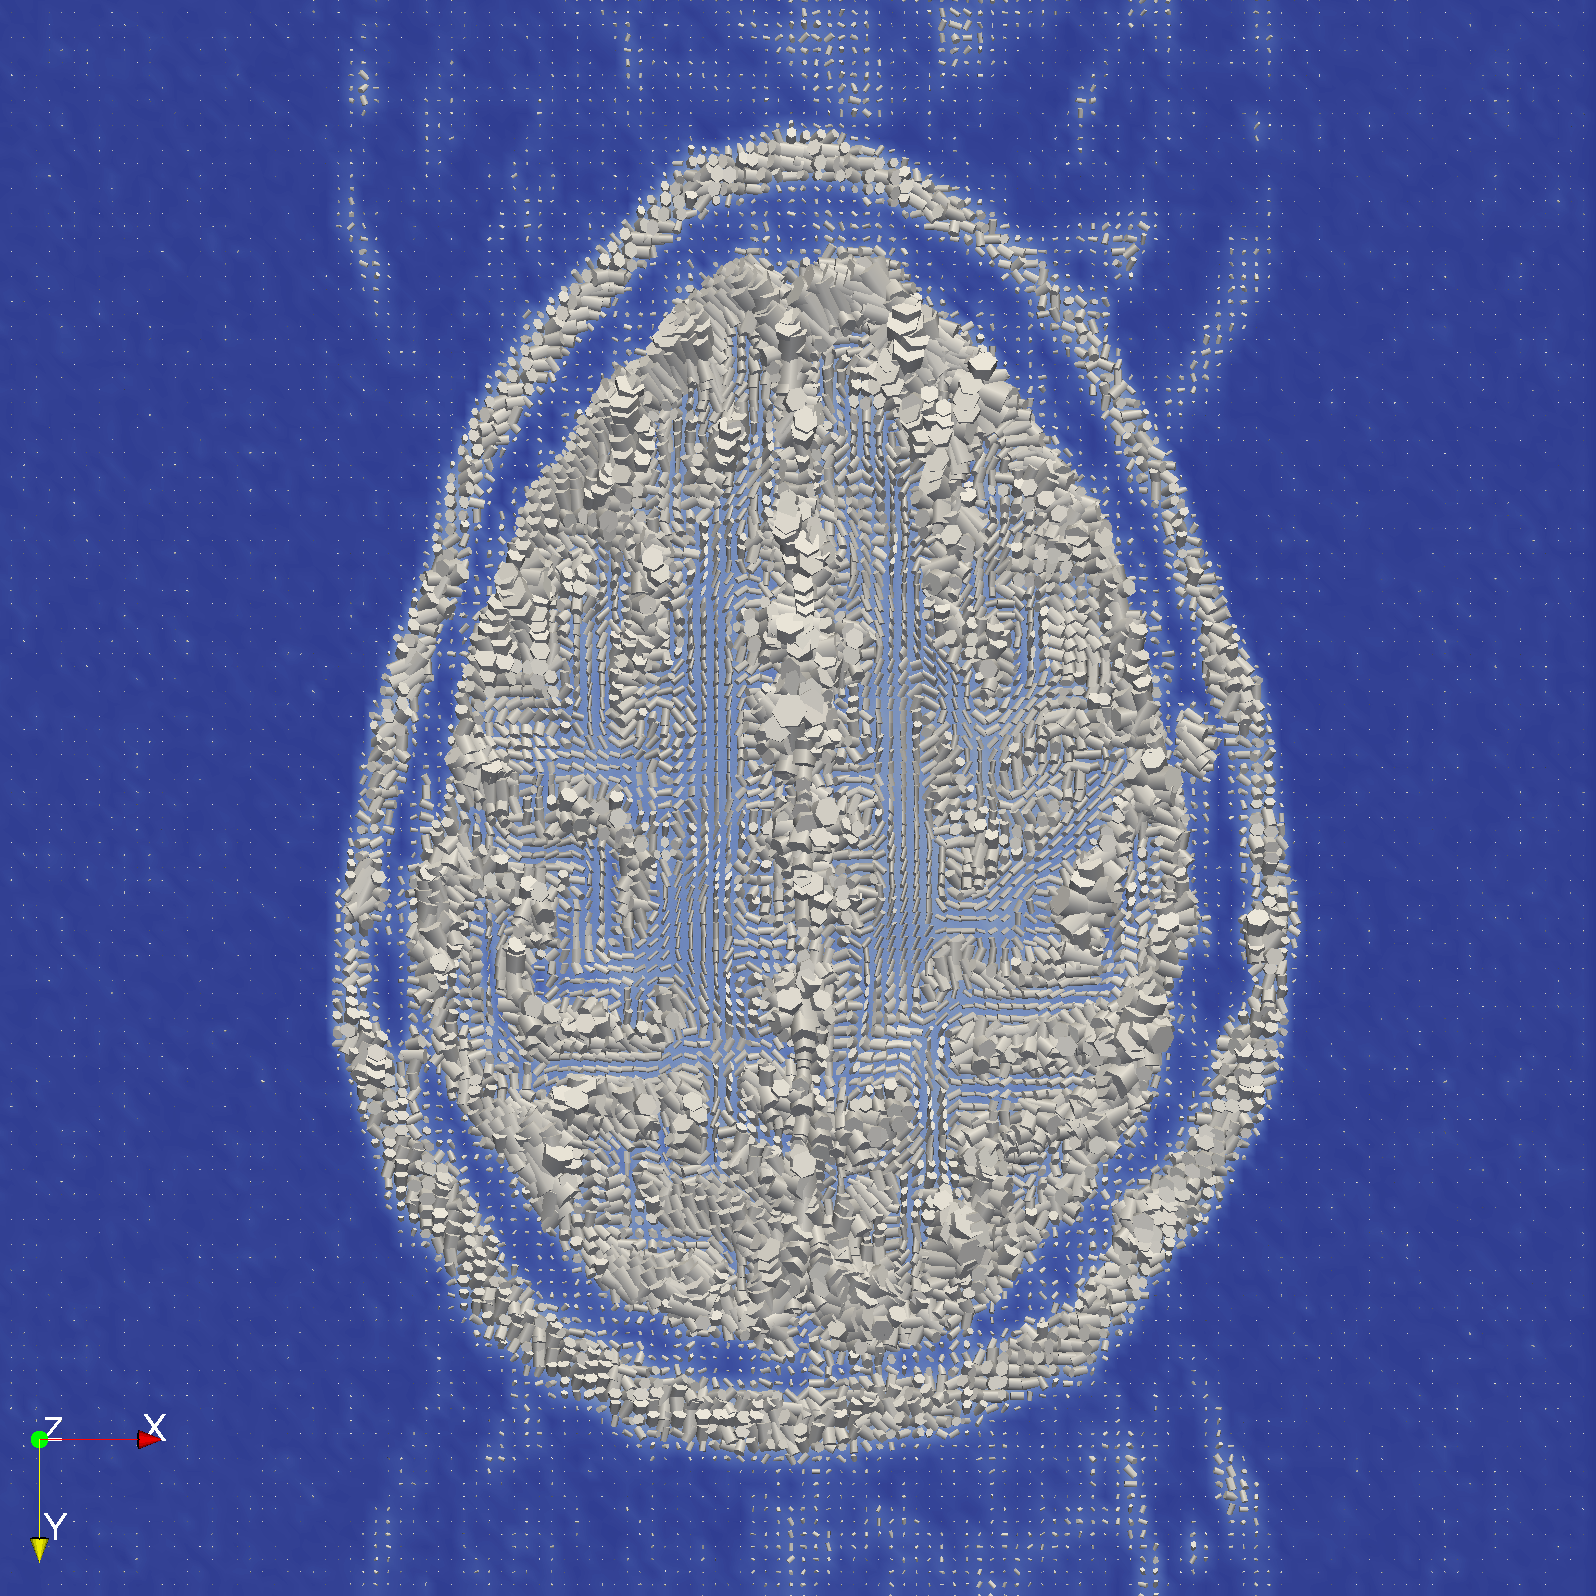
\includegraphics[width=0.8\textwidth]{img/brain_cyl_glyphs.png}
    \label{b)}
    \caption*{cyclinder glyphs}
  \end{minipage}
\caption{Real data examples: \enquote{brain} dataset}
\label{real1}
\end{figure}
Observing the \enquote{brain} dataset in Fig \ref{real1}, one may notice that it introduces a lot of variances to tensor magnitude and linear anisotropy. We choose this DTI-MRI scan as an example-par-excellence for real application data given in a reasonable resolution.
\begin{figure}[!t]
\centering
  \begin{minipage}{0.4\textwidth}
    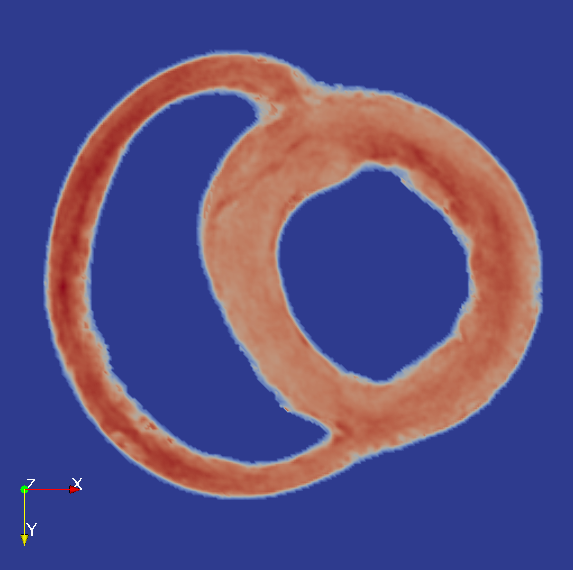
\includegraphics[width=0.8\textwidth]{img/heart_org.png}
    \label{a)}
    \caption*{tensor magnitude}
  \end{minipage}
  \begin{minipage}{0.4\textwidth}
      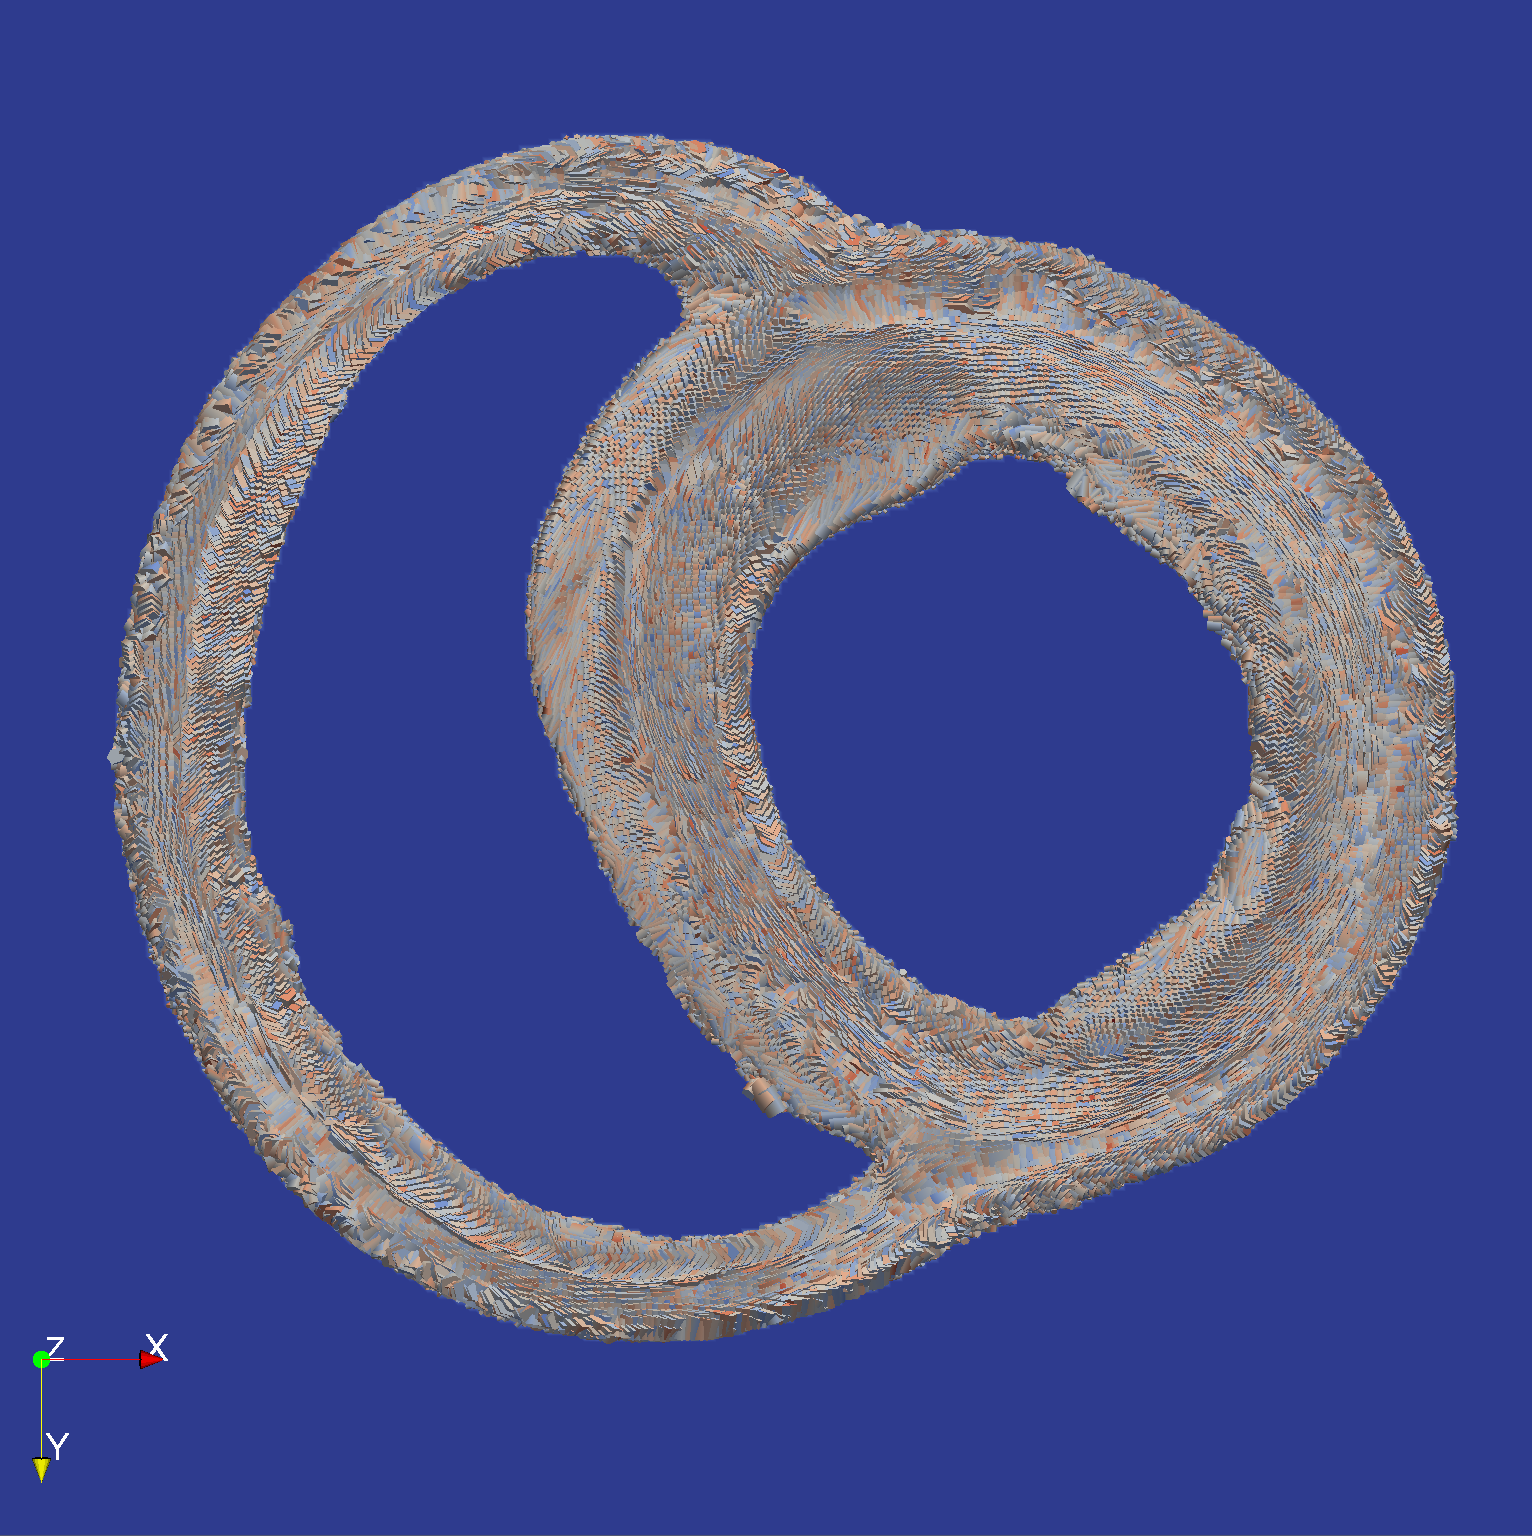
\includegraphics[width=0.8\textwidth]{img/heart_cyl_glyphs.png}
    \label{b)}
    \caption*{cyclinder glyphs}
  \end{minipage}
\caption{Real data examples \enquote{heart} dataset}
\label{real2}
\end{figure}
When we look at this DT-MRI scan of a human heart we can notice the elongated shape, which we consider to represent the aorta and a part of the rest of the heart. If we consider the glyph representation, we again infer, that we incorporate lots of anisotropic regions with varying tensor magnitudes here.


\chapter{Related Work}
\label{chap:related}

There has been extensive recent work on symmetric tensors but in comparison little on asymmetric ones. Since we are not able to cover the whole scope in this work, we will focus on the most relevant works on tensor field visualization. We will talk about the publications from Hlawatsch et al. \cite{hlawatsch} and Zirr et al. \cite{zirr} in particular, since they constitute thematically close related works. But first, we will cover related works on global illumination methods, as these form a basis or prerequisite for our work. Please note, that they do not focus on tensor field visualization at all. Remember, that we will inventively employ global illumination methods for tensor field visualization as an innovative step and that we want to cover previous works on our base approach, as well.

\paragraph{Global Illumination Methods}
Since we use a specific category of global illumination methods as a basis, we decide to only discuss lattice based methods which work, corresponding to their name, on a grid. Remark, that Global Illumination methods classically focus on realistic indirect lighting. Thus, they aim on producing a most realistic image, what in our case turns out to be a most informative image in correspondence. The most early work in this field is propably the Discrete Ordinates Method (DOM) by Chandrasekhar \cite{Chandrasekhar}, which is used specifically for computing radiative transfer in participating media (volume rendering). The radiative transfer equation is discretized spatially and in the angular domain. The radiance distribution (PDF) is stored in a grid and light is distributed and exchanged between neighboring volume elements which reduces the overall effort to local and independent computations. Furthermore, there has been more recent work on describing the light propagation as a diffusion process within a simple photon transport model based on the Lattice-Boltzmann method \cite{geist}. DOMs were recently revisited by Fattal \cite{fattal}. This work adresses artifacts stemming from spatial discretization, which are called \enquote{ray effects}, and from successive interpolation called \enquote{light smearing}. These methods are considered to be too slow to \enquote{run at interactive framerates} by Dachsbacher et al. \cite{dachsbacher}, though \enquote{efficient and potentially highly parallel}. Our work is inspired by Lattice-Boltzmann methods (volume grid radiosity) and the lattice-based discrete ordinate methods concerning the light propagation scheme.

\paragraph{Symmetric Tensor Field Visualization}
Zheng \& and Pang \cite{pang&zheng} et al. proposed a texture-based visualization approach called Hyper LIC, which extends the concept of LIC to symmetric tensor fields by using an anisotropic 2D-filter kernel oriented along the major/minor eigenvectors. The concept of following the major/minor eigenvector along tensor field lines was invented by Vilanova et al. \cite{vilanova}. Tensorlines \cite{weinstein} introduce a kind of artificial inertia (running average), making them resistent to noise. The notion of tensor field topology (critical, degenerate points, separatrices) and the concept of hyperstreamlines was first introduced by Delmarcelle and Hesselink \cite{delmarcelle&hesselink}. The topology in $3D$ tensor fields was first analyzed by Zheng et al. \cite{zheng}. The placement of tensor field lines as hyperstreamlines for glyph packing was recently improved by Spencer et al. \cite{spencer}. A good overview of seeding strategies concerning glyphs is given by McLoughlin et al. \cite{mcloughlin}. Feng et al. \cite{feng} used Voronoi Tesselation for placing the glyphs. Superquadric glyphs have been proposed by Schultz and Kindlmann \cite{schultz&kindlmann} for general (non-positive definite) tensors. De Leeuw and van Wijk \cite{deleeuw&vanwijk} visualize the partial derivative gradient, the Jacobian of the tensor field, to sense the local properties of the field. A diffusion tensor can also be visualized by box \cite{makris}, ellipsoid \cite{pierpaoli}, composite \cite{westin2} or superquadric \cite{kindlmann} glyphs. There is also a set of scalar measures available in symmetric tensor field visualization such as: mean diffusivity, fractional anisotropy \cite{basser} and anisotropy coefficients \cite{westin}. These coefficients can also be visualized by direct volume rendering \cite{kindlmann2}. Hlawatsch et al. \cite{hlawatsch} obtain a coordinate (flow) map from tensor field lines following major/minor eigenvectors (fibre trajectories) using the maximum eigenvalue of the Cauchy-Green deformation tensor to compute the FTLE-field in homogeneous regions. In a similar manner, we aim to use light transport techniques to obtain a final light distribution (flow map) through successive light propagation cycles directed (in form of transmission profiles obtained from ellipsoid glyphs) by the tensor field. DT-MRI diffusion tensor imaging can help to reveal the functional \cite{denis} or topological \cite{wakana} structure of the brain and muscles by analysing celebral and muscle tissue tractography, which yields a tensor field representing the anisotropy characteristcs of the brain's white matter. An overview about DT-MRI visualization techniques is given by \cite{vilanova}. Tricoche et al. \cite{xavier} use invariant manifolds to extract topological features from tensor fields. Other feature extraction-based approaches extract general features as: edges \cite{hancock}, tensor shape\/ orientation \cite{gordon}, interfaces \cite{donnel}, creases \cite{tricochet}.
\\
\paragraph{Asymmetric Tensor Field Visualization}
Zheng and Pang \cite{pang&zheng} proposed the concept of dual eigenvectors and Zhang et al. \cite{zhang} extended it to pseudo-eigenvectors and introduced the eigenvector/eigenvalue manifolds to visualize eigenvectors in the complex domain. Laramee et al. \cite{laramee} focused on the efficient implementation and visualization of these structures and provided an interactive visualization system for asymmetric tensors applicable in fluid and solid dynamics. The concept of tensor magnitude has been introduced by \cite{laramee} for means of physical interpretation. They also proposed an efficient glyph and hyperstreamline hybrid approach, which made dynamic interaction in real-time in $2D$ tensor fields feasible. Palacios et al. \cite{palacios} extracted isosurfaces of tensor magnitude, mode and isotropy index.

Last, we will discuss our work in relation to other publications. While these previously mentioned works use classical approaches like tensor field lines and glyphs, we will also introduce the concept of Lagrangian coherent structures into our framework contribution to tensor field analysis. LCS have been defined as time-dependent analog of separatrices \cite{haller} which are concerned to be robust under noisy conditions \cite{haller2}, which we expect from our technique as well by implication. Hlawatsch et al. \cite{hlawatsch} obtain similar results (a FTLE-like field on tensor fields), but obtain them by sampling of fiber trajectories instead of global illumination light distributions, as it is the case for this work. Our work shares the same basic idea, deriving and computing a FTLE-like field for tensor field visualization generalizing FTLE from vectors to tensors, yet using a light propagation scheme and hence using whole distributions of trajectories incorporating polar profiles. Concerning the tensor field visualization method (LTG), our approach is based on FTLE, and principal component analysis (PCA). We will detect LCS with an FTLE-derived method considering differences in final light transport distributions through computing the gradient of the resulting flow maps. The FTLE-related approach named ``light transport gradient'', to be designed, also states a generalization of the light transport visualization method FTPD proposed by Zirr et al. \cite{zirr}, since it allows a similar measure to be computed through defining a geometrical scene and setting the transmission (defined by the tensor field) to an isotropic and constant value of $100\%$. In this operating mode, the approach operates as a light transport visualization technique neglecting any tensor field transmission profiles and is thus capable of displaying bounding separatrices of a light transport scenario perturbated by obstacles \cite{zirr}. 
%Typischerweise im letzten Abschnitt dieses Kapitels wird dann auf
%verwandte Arbeiten eingegangen. Entsprechende Arbeiten sind geeignet
%zu zitieren. Beispiel: Die wurde erstmalig in den Arbeiten von Spitz
%und Gertz \cite{Spitz2016a} gezeigt \ldots Details dazu werden in
%dem Buch von Newman zu Netzwerken \cite{Newman2010} erläutert \ldots.

%%%%%%%%%%%%%%%%%%%%%%%%%%%%%%%%%%%%%%%%%%%%%%%%%%%%%%%%%%%%

% Alternative: put content in separate files
% Check the difference between including these files using \input{filename} and \include{filename} and see which one you like better
%\chapter{Einleitung}\label{intro}
%\input{introduction}
%
%\chapter{Voraussetzungen}\label{bg}
%\input{background}



\end{document}